\chapter{Implementation}
Introduction to the chapter!

\begin{figure}[!ht]
\centering
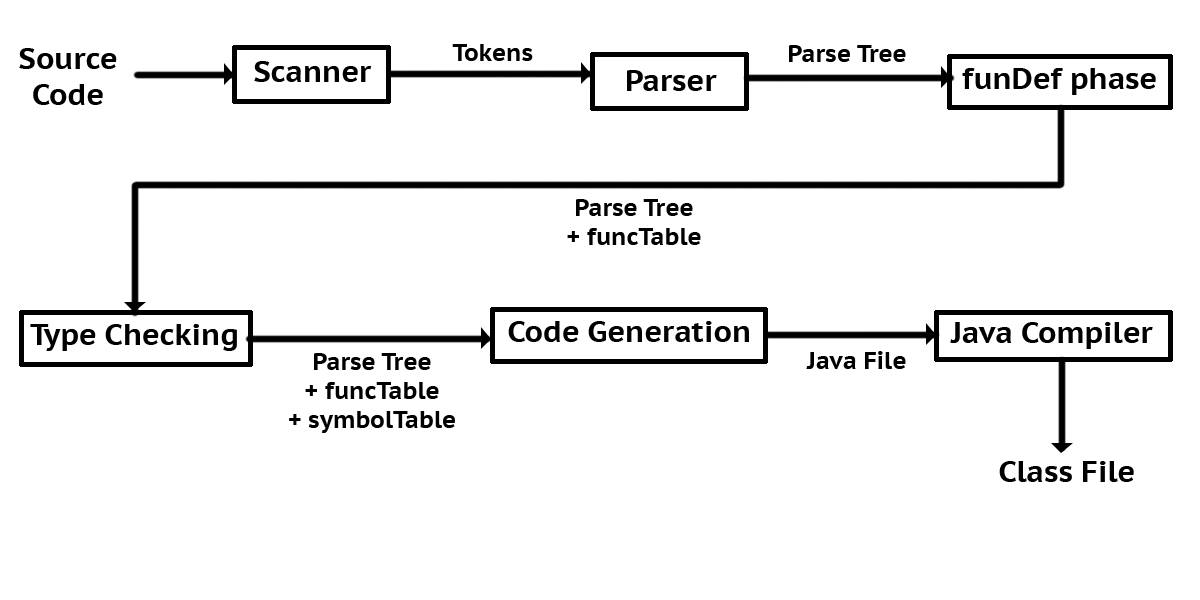
\includegraphics[scale=0.35]{billeder/compilerStructure}
\caption{Compiler structure}
\label{cs}
\end{figure}


\section{ANTLR}
Antlr og vores grammer(Tjek om vores grammar er beskrevet før)
Hvad gør antlr for os ?
Den får vores grammar og vores sourcecode, hvad gør den så ?


Forklar hvordan lexer, parser og hvordan antlr gør det. Sådan set de to første steps i diagrammet. Med deres output i form af Tokens og Parse tree.

Forklar de to visitor patterns som antlr genererer(Listener/walker og visitor)
\section{Function Definition}
After Antlr has produced the parsetree, baselistener and basevisitior, the function definition phase starts. In this phase every function that allready exists in Robocode, will be mapped to the names defined in the apendix,(Indsæt reference til apendix her!!!!!) and added to the functiontable. Also every user defined function or actions will be added to this functiontable. 

\subsection{FuncSymbol \& FuncSymbolTable}
To keep track of the varies functions and their parameters, return values and Robocode names, a FuncSymbol class is used as representation for a single function and a FuncSymbolTable class is used to keep track of every FuncSymbol in the program.
The FuncSymbol has a string properties for Name, Type, ReturnType, original Robocode names and a string array for the parameters.

The FuncSymbolTable is basically a key/value pair HashMap. Where the key is the type of the function followed by the name of the function. The type in this case, can be either Function or Action from userdefined functions, Tank, Gun, Battlefield, Radar or Utils from Robocode functions or the name of the event from Robocode events.
This class has two functions, GetFuncSymbol and EnterFuncSymbol which can be found in listing \ref{FST}. 

The GetFuncSymbol takes a type and a name from a function, combines them, looks for them in the HashMap and returns the result.

EnterFuncSymbol takes a FuncSymbol and tries to add it to the HashMap. First it checks if a function with same type and name was already declared, if such a function exists, an error is thrown, otherwise the function is added to the HashMap.

\begin{lstlisting}[caption={FuncSymbolTable}, label={FST}]
public class FuncSymbolTable {

	public LinkedHashMap<String, FuncSymbol> Map = new LinkedHashMap<String, FuncSymbol>();

	public FuncSymbol GetFuncSymbol(String type, String name){
    	FuncSymbol sym = Map.get(type + name);
    	return sym;
	}

	public void EnterFuncSymbol(FuncSymbol fs){
    	FuncSymbol oldSym = GetFuncSymbol(fs.Type, fs.Name);
    	if (oldSym != null) {
        	Error e = new Error("Function already declared");
        	throw e;
    	}
    	Map.put(fs.Type + fs.Name, fs);
	}
}
\end{lstlisting}

Forklar måden hvor på vi mapper robocode funktioner til vores funktioner
Forklar om den listener og walker vi bruger og hvordan de virker. (I hvert fald  få forklaret hvodan vi implementere dem her, hvis de er beskrevet  i den section før)
Error handling
Forklar om de to forskellige functables der bliver generete af henholdsvis bruger og fra den fil der bilver loadet ind. 

\subsection{Robocode functions \& events}
To allow the typechecker and codegeneration phase to do their jobs, every Robocode function and event needs to be added to the FuncSymbolTable. To do this a simple textfile was created which line for line have each function written out in a specific manner. 

WE COULD EXPLAIN THE TEXTFILE AND THE ALGORITHM USED TO LOAD IT IN IF WE HAVE TIME!!

\subsection{Userdefined Functions \& Actions}
To load the user defined functions from the program, a traverse of the parse tree is done using the Antlr generated walker/listener. For every Function and Action the listener visits, a new FuncSymbol is created and added to the FuncSymbolTable. This is done with the FuncListener class, which extends the BaseListener Antlr created.
 
The FuncListener class overrides the Enter/Exit Action declaration functions, the Enter/Exit Function declaration functions and the Enter parameter function. In the Enter Action and Function declaration functions, a new FuncSymbol is created called CurrentFunc. To CurrentFunc a name and a type is added, and in the Function case a return type is added aswell. Name, type and return type are found using the parse tree.
In the Enter parameter function adds a new parameter to the CurrentFunc's array of parameters. 
Now in the Exit Action and Function declaration functions the CurrentFunc gets added to the FuncSymbolTable. 
The reason the CurrentFunc is added in the Exit functions, is that the walker have to visit all the parameters. 

\section{Type checking} 
After the first travesal of the parse tree using the FuncListener, every function is now defined in the function table and we can begin type checking. To do type checking a Symbol- and a SymbolTable class are used to keep track of every variable and their scope, using these two classes the SymbolTypeVisitor class checks for type compatibility. 

\subsection{Symbol \& Symbol table}
Every variable in the program is represented by the Symbol class. The Symbol class has the properties String Name and Type, Symbol Var and int Depth. The Name and Type represents the name and type of the variable, the interesting parts is the Var and Depth properties. Var is a reference to a Symbol of the same name but in a higher scope, this would work as stack for all symbols of the same name, where the top of the stack will be the most inner scope and therefore the one used. The Depth property indicates the depth of the scope the symbol is in, with 0 being the global scope. 

The SymbolTable is mainly two things, the Map associates a name of a variable with a symbol as key value pairs, these symbols are the ones on top of the stack describes in the paragraph before. The scope is an array of arrays of symbols. Each index of the outer array is a scope and each inner array contains the symbols of that scope. 

The SymbolTable class has four functions: OpenScope, CloseScope, GetSymbol and EnterSymbol. 

OpenScope in listing \ref{OS} is used to open a new scope. Depth is a global variable, which keeps track of the current scope's depth. When OpenScope is run, the depth is incremented. If the Scope size is less than the depth + 1, a new array is added to the scope, otherwise the old array is cleared.

\begin{lstlisting}[caption={OpenScope function}, label={OS}]
public void OpenScope(){
    depth++;
    if (Scope.size() < depth+1){
        Scope.add(new ArrayList<Symbol>());
    }else {
        Scope.get(depth).clear();
    }
}
\end{lstlisting}

 The EnterSymbol function in listing \ref{ES}, is used to enter e new symbol into the SymbolTable. When EnterSymbol is run it firstly checks if there already exists a symbol with the same name, if this is the case it checks whether the depth of this symbol is the same depth as current scope. If the depths are the same, an error is thrown, since there can't exist two variables with the same name in the same scope. If no symbol exists in the Map or it is at another depth, a new symbol is created. This symbol gets the current depth in its depth property and it sets its var property to the old symbol. It then either replaces the new symbol with the old symbol or just adds it if the old symbol was null. 

The GetSymbol function looks up a symbol in the map and will return the name of that symbol.

\begin{lstlisting}[caption={EnterSymbol function}, label={ES}]
public void EnterSymbol(String name, String type){
    Symbol oldsym = Map.get(name);
    if (oldsym != null && oldsym.Depth == depth){
        Error e = new Error("Duplicate declaration of " + name);
        throw e;
    }else{
        Symbol newSym = new Symbol();
        newSym.Name = name;
        newSym.Type = type;
        newSym.Depth = depth;
        newSym.Var = oldsym;
        Scope.get(depth).add(newSym);
        Map.put(newSym.Name, newSym);
    }
}
\end{lstlisting}

CloseScope in listing \ref{CS}, is used to close the current scope. This is done by going through each symbol \textbf{s} at the current depth, and replacing \textbf{s} in the Map with \textbf{s.Var} which is a symbol with the same name but in a higher scope. If no such symbol exists, \textbf{s} is replaced with a null value. 

\begin{lstlisting}[caption={CloseScope function}, label={CS}]
public void CloseScope(){
        Scope.get(depth).forEach(s -> {
            Symbol prevSym = s.Var;
            Map.replace(s.Name, s, prevSym);
        });
        depth--;
    }
\end{lstlisting}



\subsection{The SymbolTypeVisitor class}


Forklar vi "overskriver" visitoren, eller vi bruger visitoren.
\section{Code generation}


\section{Compiling}


TO DO
Rename Txt og TEXT til String.
Open og close scope i functionBlockContext
CodeGen errors
Ændre while i codegen
Lav billede til Environment store model, og forklar det!
Apendix, skriv tekst til det vi har, overvej om der skal tilføjes kode eksempler.
Formuler en problem stilling i introduction.


